\documentclass[10pt]{beamer}%t: top aligned frames
%[hyperref={colorlinks, citecolor=hltyellow,linkcolor=hltdarkgreen,
  %urlcolor=hltdarkgreen}]
\usepackage[T1]{fontenc}
\usepackage[utf8]{inputenc}
\usepackage[english]{babel} % [magyar]
\usepackage[backend=bibtex,natbib=true,style=authoryear,backref=true]{biblatex}%autocite=superscript
\renewcommand*{\bibfont}{\footnotesize}
\bibliography{../../paper/Common/Bib/ml}
\usepackage{lmodern}
\usepackage{booktabs}
\usepackage{mathabx}
\usepackage{amsmath}
%\usepackage{mathtools}
%\usepackage[all]{xy}
\usepackage{graphicx}
\usepackage{tikz}
\usepackage{balance}
\usepackage{tikz-qtree}
\usepackage{longtable}
\usepackage{multirow}
\usepackage{mathtools}
%\usepackage{adjustbox}

\usepackage{pgfplots}
\pgfplotsset{%compat=1.11,
  /pgfplots/ybar legend/.style={
    /pgfplots/legend image code/.code={%
      %\draw[##1,/tikz/.cd,yshift=-0.25em]
      %(0cm,0cm) rectangle (3pt,0.8em);},
      \draw[##1,/tikz/.cd,bar width=3pt,yshift=-0.2em,bar shift=0pt]
      plot coordinates {(0cm,0.8em)};},
    },
}
\usetheme{hlt}
%\usecolortheme{rose}
%\definecolor{hltblue}{RGB}{3,61,92}
\definecolor{hltdarkgreen}{RGB}{26,148,129}
%\definecolor{hltlightgreen}{RGB}{155,204,147}
%\definecolor{hltyellow}{RGB}{252,238,166}
%\usecolortheme[named=hltblue]{structure}
%\setbeamercolor{alerted text}{fg=hltdarkgreen}
%\setbeamercolor{example text}{fg=hltlightgreen}

%work-around for citation colour with Beamer + Hyperref + Natbib
\let\oldbibitem=\bibitem
\renewcommand{\bibitem}[2][]{\label{#2}\oldbibitem[#1]{#2}}
\let\oldcite=\cite
%\renewcommand\cite[1]{\hypersetup{linkcolor=hltblue} \hyperlink{#1}{\oldcite{#1}}}
\let\oldcitep=\citep
%\renewcommand\citep[1]{\hypersetup{linkcolor=hltblue}\hyperlink{#1}{\oldcitep{#1}}}
\let\oldciteauthor=\citeauthor
%\renewcommand\citeauthor[1]{\hypersetup{linkcolor=hltblue}\hyperlink{#1}{\oldciteauthor{#1}}}

\newcommand{\bull}[1]{\begin{itemize}\item #1 \end{itemize}}
\newcommand{\fl}{\texttt{4lang}}
\newcommand{\jiweil}{\texttt{mutli}}
\newcommand{\huang}{\texttt{huang}}
\newcommand{\neela}{\texttt{neela}}
\newcommand{\adagram}{\texttt{AdaGram}}
\newcommand{\mutli}{\texttt{mutli}}
\newcommand{\osub}{\texttt{OSub}}

\newcommand{\Ro}{\mathbb{R}^{d_1}}
\newcommand{\Rt}{\mathbb{R}^{d_2}}
\newcommand{\any}{\texttt{lax}}
\newcommand{\disamb}{\texttt{disamb}}
\newcommand{\e}{$^E$}
\newcommand{\id}{$^I$}
\newcommand{\s}{$^S$}

\author{Márton Makrai}
\title{%Do
  Multi-sense word embeddings}%learn more senses?}
\logo{\includegraphics[width=1cm]{../../paper/Common/Logo/nytud/nytud}}
%[Makrai Márton]{
%  Makrai Márton \\
%\vspace{5mm}
%\hspace{5mm}
%  }
\date{K + K = 120 Workshop}
%[Fiatal kutatók félidőben 2017]{
%  témavezető: Kornai András\\
%    \vspace{2mm}
%  Fiatal kutatók félidőben \\
%2017. szeptember 28.}
\begin{document}
\AtBeginSection[]{
  \begin{frame}{Overview}
    \tableofcontents[currentsection,subsectionstyle=shaded]
  \end{frame}
}

\maketitle


\begin{frame}{Overview}
  \tableofcontents
\end{frame}

% a) a témát, a releváns hazai és nemzetközi szakirodalmat (20%) 3 dia
% b) kutatásának célját, a kutatási kérdéseket, a hipotéziseket (5%) 1 dia
% c) módszertant, amelyre a kutatás épül (20%) 3 dia
% d) eredményeket (ahol lehet, szemléltesse ábrákkal) (35%) 5 dia
% e) következtetéseket, amelyek az eredmények alapján levonhatók (18%) 2 dia
% f) Az előadást záró diaképen összegezze eddigi publikációit

\section{Word embeddings}

\begin{frame}{Artificial neural networks}
\centering\includegraphics[width=.7\textwidth]{../../paper/misc/makrai/fiatal/felido/img/deep_neural_network}
  \begin{itemize}
    \item cybernetics (1949), connectionism (1974), deep learning (2006)
    \item Learning features, more and more abstract layers
    \item
      \begin{itemize}
        \item computer vision \citep{Krizhevsky:2012}
        \item speech recognition \citep{Hinton:2012}
      \end{itemize}
    \item fast learning on the graphics card
    \item like in the brain?
  \end{itemize}
\end{frame}

\begin{frame}{Word embeddings}
  \begin{itemize}
    \item Representation of words in neural networks
    \item $\mathbf w \in \mathbb R^{300}$
    \item words with similar distribution $\leadsto$ similar points
    \item unsupervised training on giga-word corpora
      %TODO Data \cite{Halácsy:2004,Oravecz:2014}
    \item word2vec: skip-gram or continuous bag of words \\ \citep{Mikolov:2013d}
    \item representation sharing \\ \citep{Collobert:2011,Hashimoto:2017}
    \item compositionality \\ character, morph, word, query, sentence, rhetorics
      \begin{itemize}
        \item morphs \citep{Lazaridou:2013}
        \item bellow the word level: fastText \citep{Bojanowski:2016}
        \item thought vector \citep{Vaswani:2017}
      \end{itemize}
  \end{itemize}
\end{frame}

\begin{frame}{Meaning decomposition with vectors}
  \cite{Katz:1963,Mikolov:2013l}
  \includegraphics[width=\textwidth]{../../paper/misc/makrai/fiatal/felido/img/analogy}
  \[ \text{\bf king} + \text{\bf woman} - \text{\bf man} \approx \text{\bf queen}\]
      \begin{itemize}
        \item nearest neighbors
        % \item other relationships?
      \end{itemize}
\end{frame}

\begin{frame} {Word translation (Mikolov et al., \citeyear{Mikolov:2013x})}
  \begin{columns}
    \begin{column}{.65\textwidth}
  \begin{itemize}
    \item linear mapping between embeddings, 600 $\rightarrow$ 300 dim
      %\\ the simplest between two vector spaces
      %\item now embedding two languages
    \item training on the 5~000 most frequent pairs  \\
    \item test on the next 1~000
  \end{itemize}
    \end{column}
    \begin{column}{.4\textwidth}
      \begin{align*}
        W : \Ro \rightarrow \Rt \quad z\approx Wx \\
        \min_W \sum_i || Wx_i - z_i &|| ^ 2
      \end{align*}
    \end{column}
  \end{columns}
    \begin{figure}
      \includegraphics[width=\textwidth]{../../paper/misc/makrai/fiatal/skip_gram_mapping}
    \end{figure}
\end{frame}

\section {Multi-sense}

\begin{frame}{Word ambiguity}
  \begin{itemize}
    \item homonymy: Russian \emph{mir} `world'; `peace'
    \item polysemy: Hungarian \emph{nap} `Sun; day'
    \item evidence for differentiation
      \begin{itemize}
        \item etymology: common origin
          \begin{itemize}
            \item uncertain for many words
            \item how far back?
          \end{itemize}
        \item relatedness of meanings (intuition. Agreement?)
        %\item part-of-speech (Hungarian \emph{vár} `wait'; `castle')
      \end{itemize}
  \end{itemize}
  \begin{tabular} {lll}
    \toprule
    disambiguation (WSD) & classification & supervised \\
    induction (WSI) \citep{Schutze:1998} & clustering & unsupervised \\
    \bottomrule
  \end{tabular}
      %\item polysemy graphs,
      %\begin{itemize}
      %\item which terms tend to be polysemous
      %\item similarities between languages  \cite{Youn:2016}
      %\item concept clusters
      %\end{itemize}
      %\item sup-types of polysemy
      %\begin{tabular}{llll}
      %\toprule
      %metonymy & regular    & \emph{school} (people, building -- both
      %literal) \\
      %metaphor & irregular  & \emph{eye}
      %(lit `organ' $\leadsto$ fig `hole in needle') \\
      %\bottomrule
      %\end{tabular}
\end{frame}

\begin{frame}{Multi-sense vector models}
  \begin{itemize}
    \item multi-``prototype'' embeddings \citep{Reisinger:2010}
    \item with neural network \citep{Huang:2012}
    \item multi-sense skip gram, open-source tools
      \begin{itemize}
        \item \cite{Neelakantan:2014}
        \item as a Dirichlet Process
          \begin{itemize}
            \item \adagram~\citep{Bartunov:2015}
            \item \mutli~\citep{Li:2015}
          \end{itemize}
      \end{itemize}
      %\item still in the research phase
    \item if the number of parameters is controlled \citep{Li:2015}
      \begin{itemize}
        \item slight performance boost in
          \begin{itemize}
            \item semantic similarity for words and sentences,
            \item semantic relation identification,
            \item part-of-speech tagging
          \end{itemize}
        \item no improvement in
          \begin{itemize}
            \item sentiment analysis
            \item named entity extraction
          \end{itemize}
      \end{itemize}
    \item sense resolution is too fine (duplicates)
  \end{itemize}
\end{frame}


% TODO distribution of the number of senses

\begin{frame}{Linear translation from multi-sense embedding}
  \begin{itemize}
    \item Borbély, Makrai, Nemeskey, and Kornai \citeyear{Borbely:2016}
    \item principle: homonymous senses $\leadsto$ different translations
    \item target embedding remains single-sense \\
      \citep{Pennington:2014,Mikolov:2013f}
  \end{itemize}
          \begin{figure}
            \centering
            \resizebox{\textwidth} {!} {%
              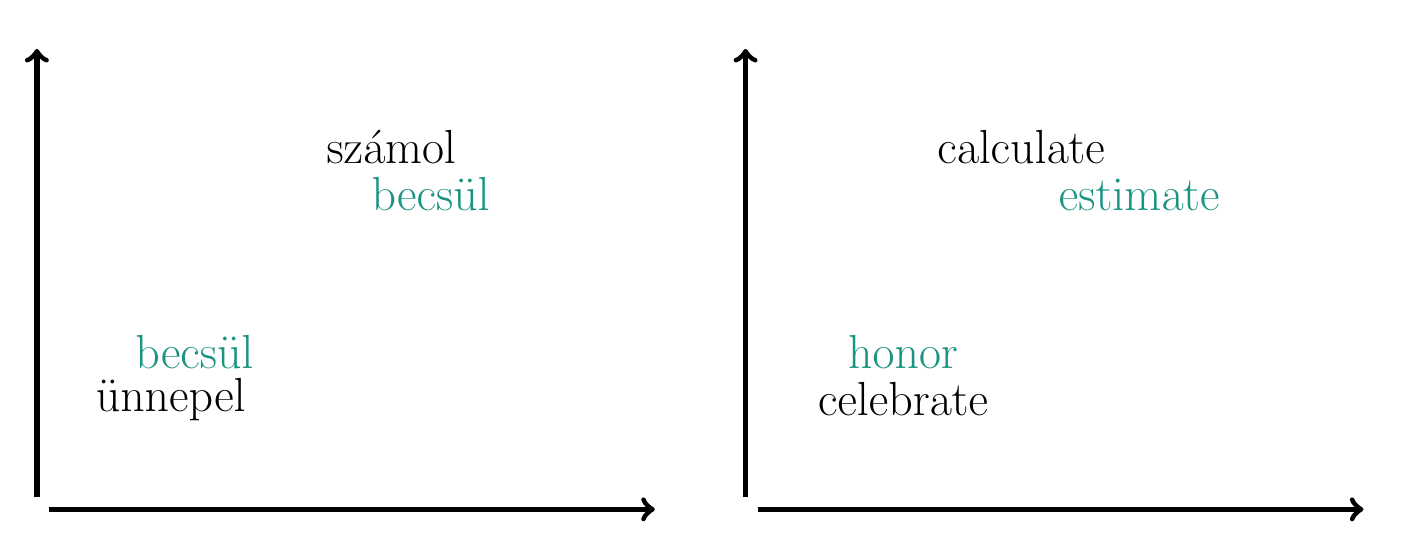
\begin{tikzpicture}[line width=2pt] %[&gt;=stealth']
                \tikzstyle{every node}=[font=\LARGE]
                %\tikzset{every edge thick}
                \node[text=hltdarkgreen] (hf) at (2, 2) {becsül};
                \node (hf) at (1.7, 1.4)  {ünnepel};
                \node[text=hltdarkgreen] (hs) at (5, 4)  {becsül};
                \node (hs) at (4.5, 4.6)  {számol};
                \node[text=hltdarkgreen] (gf) at (11, 2) {honor};
                \node (gf) at (11, 1.4) {celebrate};
                \node[text=hltdarkgreen] (gs) at (14, 4) {estimate};
                \node (gs) at (12.5, 4.6) {calculate};
                \node (ho) at (0, 0) {};
                \node (hx) at (8, 0) {};
            \node (hy) at (0, 6) {};
            \node (go) at (9,0) {};
            \node (gx) at (17,0) {};
            \node (gy) at (9,6) {};

            \draw[->] (ho) edge (hx);
            \draw[->] (ho) edge (hy);
            \draw[->] (go) edge (gx);
            \draw[->] (go) edge (gy);
          \end{tikzpicture}
        }
        % \caption{Linear translation of word senses. The Hungarian word
        % \emph{honor} is ambiguous between `honor 'and' estimate'.}
        % \label{fig: AdaGram}
      \end{figure}
\end{frame}

\section{Experiments}

\begin{frame}{Data}
  \begin{itemize}
    \item source corpus
      \bull{
      de-glutinized version \citep{Borbely:2016d,Nemeskey:2017} of the
      % Borbely Kornai Kracht Nemeskey
      Hungarian National Corpus \citep{Oravecz:2014}}
    \begin{center}
        \resizebox{\textwidth} {!} {%
      \begin{tabular}{rcll}
         \texttt{jelmondatával} & $\rightarrow$ & \texttt{jelmondat <POSS> <CAS<INS>>} & `(with its) motto'\\
    \texttt{akartak} & $\rightarrow$ & \texttt{akar <PAST> <PLUR>} & `(they)
      want(ed)'\\
      \end{tabular}
      }
    \end{center}
    \item target embedding: GloVe 840B 300d \citep{Pennington:2014}
    \item seed dictionary: wikt2dict \citep{Acs:2013}
    \item training on the first meaning
    %\item target restricted to 20--62 K words
  \end{itemize}
\end{frame}

\begin{frame}{Examples}
        \resizebox{\textwidth} {!} {%
  \begin{tabular}{lllll}
    \toprule
       & sim & & covg \\
    \midrule
      S	& 0.0974	& kapcsolat	& affair, conjunction, linkage	& 0.33 \\
      S	& 0.136	& futó	& runner, bishop	& 1.0 \\
      I	& 0.1361	& kocsi	& coach, carriage	& 1.0 \\
      S	& 0.1626	& fogad	& bet, greet	& 1.0 \\
      S	& 0.1873	& induló	& march, candidate	& 1.0 \\
      S	& 0.2052	& zavar	& disturbance, annoy, disturb, turmoil	& 0.57 \\
      S	& 0.2206	& bemutató	& exhibition, presenter	& 0.67 \\
      I	& 0.2494	& gazda	& farmer, boss	& 0.67 \\
      I	& 0.2506	& kapu	& gate, portal	& 1.0 \\
      I	& 0.2515	& előbbi	& anterior, preceding	& 0.67 \\
      I	& 0.2558	& kötelezettség	& engagement, obligation	& 0.67 \\
      S	& 0.2807	& sorozat	& suite, serial, succession	& 1.0 \\
      S	& 0.2935	& durva	& coarse, gross	& 0.18 \\
      I	& 0.3097	& megkülönböztetés	& discrimination, differentiation	& 0.5 \\
      I	& 0.319	& hirdet	& advertise, proclaim	& 1.0 \\
      I	& 0.3299	& aláírás	& signing, signature	& 0.67 \\
    \bottomrule
  \end{tabular}
  }
\end{frame}

%\begin{frame}{Evaluation metrics}
\begin{frame}{The resolution trade-off}
  \begin{itemize}
    \item different vectors $ \xRightarrow ? $ different meanings
    \item \any: selection of parameters and target embedding
      \bull{at least one meaning vector should have a good translation}
    \item \disamb: different sense vectors should have a different set of good
      translations
        \bull{ratio of such items among those predicted to be ambiguous}
        % TODO cikket hozzáolvasni a Table 3-hoz tartozó szövegtől
  \end{itemize}
      \begin{table}[allowframebreaks]
        % \Resizebox {\columnwidth} {!} {%
        \begin{tabular}{lcc}
          \toprule
                                    & \any     & \disamb \\
          \midrule
          \adagram                  & 73.3\%  & 18.53\% \\
          \mutli~``sense vectors''  & 71.0\%  & 19.46\% \\
          \mutli~``context vectors''& 69.9\%  & {\bf 20.76\%} \\
          \bottomrule
        \end{tabular}
        %}
      \end{table}
      \[p(w_i\mid w_j) \, \propto \, \exp (u_i ^\top v_j)\]
\end{frame}

\begin{frame}{Problem: synonymous translations}
  \begin{figure}
    \centering
      \resizebox{\textwidth} {!} {%
        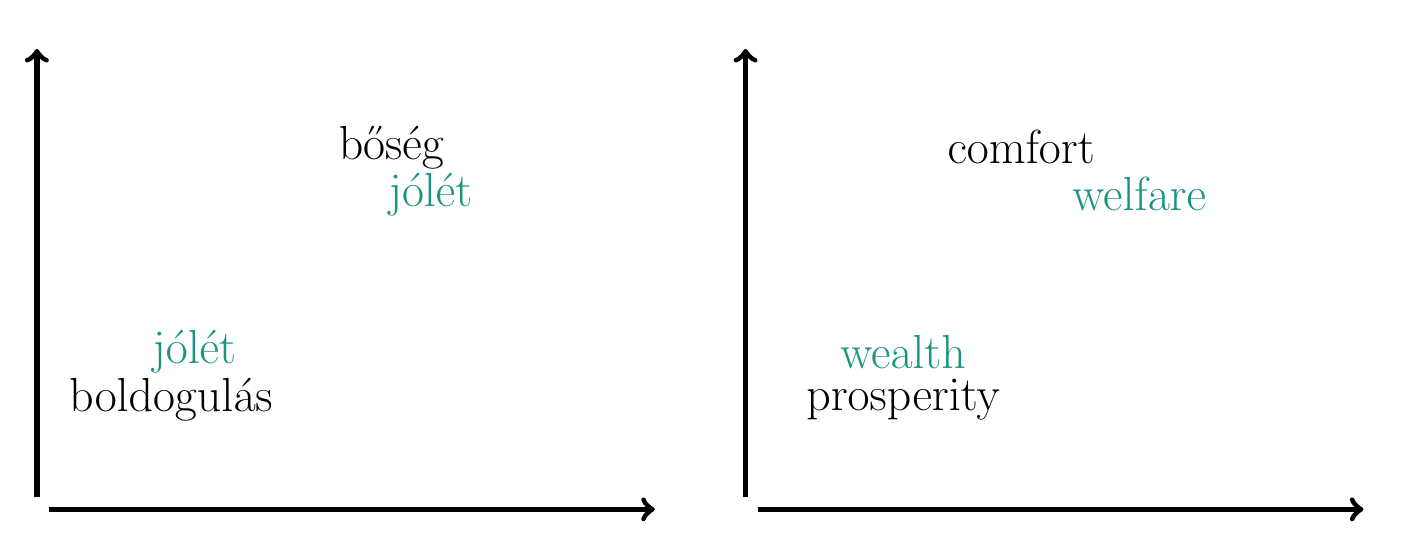
\begin{tikzpicture}[line width=2pt] %[&gt;=stealth']
          \tikzstyle{every node}=[font=\LARGE]
          %\tikzset{every edge thick}
          wealth', 'prosperity'], ['welfare', ''], ['', '], [''], [''], ['comfort
            \node[text=hltdarkgreen] (hf) at (2, 2) {jólét};
            \node (hf) at (1.7, 1.4)  {boldogulás};
            \node[text=hltdarkgreen] (hs) at (5, 4)  {jólét};
            \node (hs) at (4.5, 4.6)  {bőség};
            \node[text=hltdarkgreen] (gf) at (11, 2) {wealth};
            \node (gf) at (11, 1.4) {prosperity};
            \node[text=hltdarkgreen] (gs) at (14, 4) {welfare};
            \node (gs) at (12.5, 4.6) {comfort};
            \node (ho) at (0, 0) {};
            \node (hx) at (8, 0) {};
            \node (hy) at (0, 6) {};
            \node (go) at (9,0) {};
            \node (gx) at (17,0) {};
            \node (gy) at (9,6) {};

            \draw[->] (ho) edge (hx);
            \draw[->] (ho) edge (hy);
            \draw[->] (go) edge (gx);
            \draw[->] (go) edge (gy);
        \end{tikzpicture}
      }
      % \caption{Linear translation of word senses. The Hungarian word
      % \emph{honor} is ambiguous between `honor 'and' estimate'.}
      % \label{fig: AdaGram}
  \end{figure}
\end{frame}

\begin{frame}{Happy Birthday!}{Some of the most ambiguous 25 words}
  % do head -25 $file|shuf -n 8|sort  -t'    ' -gk2
        \resizebox{\textwidth} {!} {%
		\begin{tabular}{lllll}
			%\setlength{\tabcolsep}{3pt}
			%\centering
			\toprule
			& & sim & & covg \\
			\midrule
			\multirow{8}{*}{\rotatebox[origin=c]{90}{\mutli~``context vs''}}
			&sokaság	& 0.07848	& plurality crowd multitude	& 0.38 \\
			&kar	& 0.1008	& arm choir	& 1.0 \\
			&alkalmazás	& 0.1087	& adaptation hiring employ app	& 0.67 \\
			&bejelent	& 0.1119	& announce lodge	& 1.0 \\
			&csomó	& 0.116	& lump mat knot	& 1.0 \\
			&összeállítás	& 0.1247	& binding compilation editing composition	& 0.8 \\
			&agy	& 0.1746	& butt hub	& 1.0 \\
			&találkozó	& 0.1898	& reunion appointment	& 1.0 \\
			\midrule
			\multirow{8}{*}{\rotatebox[origin=c]{90}{\adagram}}
			&fordítás	& 0.06056	& turning compilation translation	& 0.75 \\
			&ruha	& 0.1154	& dress costume rig clothes garment	& 0.62 \\
			&alkalmazás	& 0.1236	& app employ	& 0.33 \\
			&törzs	& 0.1308	& tribe stem trunk waist hull	& 0.62 \\
			&függő	& 0.145	& dependent aerial addict	& 0.6 \\
			&hangsúlyoz	& 0.1595	& stress accent	& 0.67 \\
			&nyom	& 0.2582	& clue squeeze weigh hint push trace slot foil	& 0.62 \\
			&mag	& 0.2634	& kernel seed	& 0.4 \\
			\bottomrule
		\end{tabular}
    }
\end{frame}

\begin{frame} [allowframebreaks] {Bibliography}
	\printbibliography
\end{frame}

\begin{frame}[allowframebreaks]{Number of senses against frequency}
  %{Dirichlet Process}
  \begin{figure}
    \includegraphics[width=\textwidth]{img/adagram.pdf}
    \caption{\adagram~\citep{Bartunov:2015}}
  \end{figure}
  Ambiguity jumps at frequency 90.


  \begin{figure}
  \includegraphics[width=\textwidth]{img/mutli-full-vocab.pdf}
    \caption{\mutli, Chinese Restaurant Process \citep{Li:2015}}
  \end{figure}

  \begin{figure}
  \includegraphics[width=\textwidth]{img/mutli-top-10k.pdf}
    \caption{\mutli, top 10 K word senses}
  \end{figure}
\end{frame}

\begin{frame}{Reverse nearest neighbors}
  \begin{itemize}
    \item nearest neighbor (NN) search in high-dimensional spaces $\leadsto$
    \item \emph{hubs}, data points that are NNs of many points
      \bull{wrong in most of the cases  \citep{Radovanovic:2010}}
    \item solution: reverse nearest neighbor (revNN) queries \\ \citep{Korn:2000}
    \item reverse neighborhood rank
      \bull{\emph{project} is a $k$th revNN of \emph{work}
      $\xLeftrightarrow\Delta$
      \emph{work} is the $k$th NN of \emph{project}}
    \item there may be zero, one, or more $k$th revNNs of a word
    \item revNN query: return the words with the lowest revNN ranks
    \item less prone to hubs
    \item in linear translation \citep{Dinu:2015,Lazaridou:2015}
  \end{itemize}
\end{frame}

\end{document}
